\documentclass[ignorenonframetext,aspectratio=169]{beamer}
\usetheme{guadec}
\usepackage{amssymb,amsmath}
\usepackage{ifxetex,ifluatex}
\usepackage{fixltx2e} % provides \textsubscript
\ifxetex
  \usepackage{fontspec,xltxtra,xunicode}
  \defaultfontfeatures{Mapping=tex-text,Scale=MatchLowercase}
\else
  \ifluatex
    \usepackage{fontspec}
    \defaultfontfeatures{Mapping=tex-text,Scale=MatchLowercase}
  \else
    \usepackage[utf8]{inputenc}
  \fi
\fi
\usepackage{graphicx}
% Redefine \includegraphics so that, unless explicit options are
% given, the image width will not exceed the width of the page.
% Images get their normal width if they fit onto the page, but
% are scaled down if they would overflow the margins.
\makeatletter
\def\ScaleIfNeeded{%
  \ifdim\Gin@nat@width>\linewidth
    \linewidth
  \else
    \Gin@nat@width
  \fi
}
\makeatother
\let\Oldincludegraphics\includegraphics
{%
 \catcode`\@=11\relax%
 \gdef\includegraphics{\@ifnextchar[{\Oldincludegraphics}{\Oldincludegraphics[width=\ScaleIfNeeded]}}%
}%

% Comment these out if you don't want a slide with just the
% part/section/subsection/subsubsection title:
\AtBeginPart{
  \let\insertpartnumber\relax
  \let\partname\relax
  \frame{\partpage}
}
\AtBeginSection{
  \let\insertsectionnumber\relax
  \let\sectionname\relax
  \frame{\sectionpage}
}
\AtBeginSubsection{
  \let\insertsubsectionnumber\relax
  \let\subsectionname\relax
  \frame{\subsectionpage}
}

\setlength{\parindent}{0pt}
\setlength{\parskip}{6pt plus 2pt minus 1pt}
\setlength{\emergencystretch}{3em}  % prevent overfull lines
\setcounter{secnumdepth}{0}

\title{Automated tests for Gnome-logs}
\author{Rashi Aswani}

\begin{document}
\frame{\titlepage}

\begin{frame}

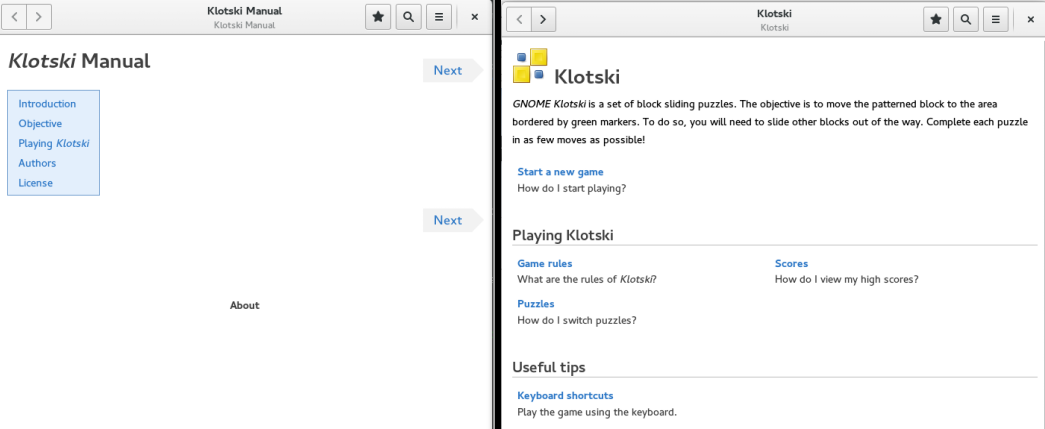
\includegraphics[scale=0.5]{klotski1.png}\\ ---

\end{frame}

\begin{frame}

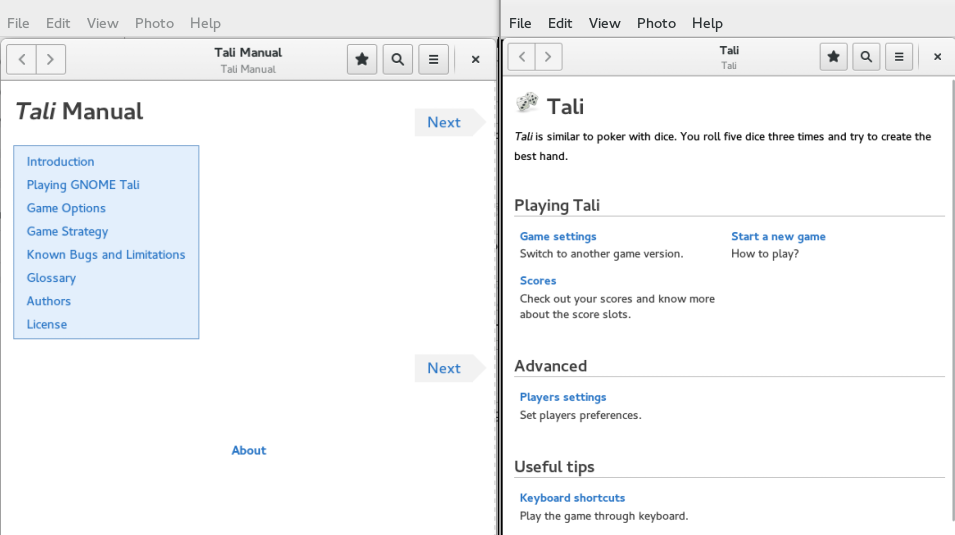
\includegraphics{Tali_picture.png}\\ ---

\end{frame}

\begin{frame}{GNOME Logs}

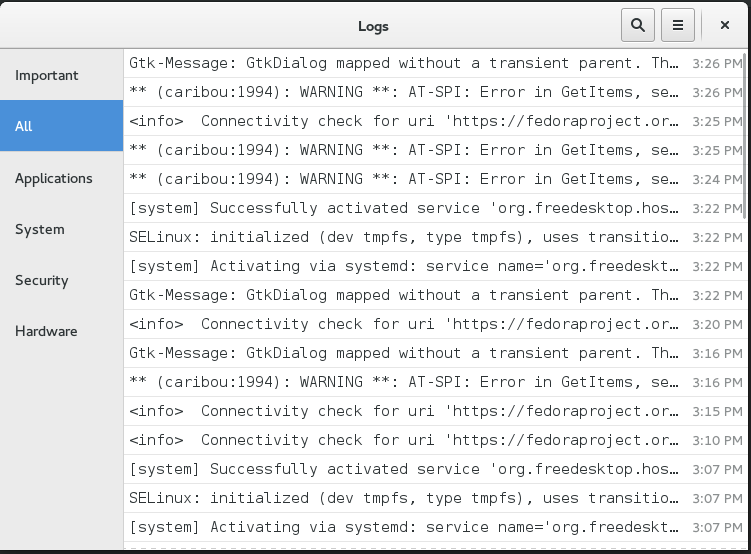
\includegraphics{logs.png}\\

\end{frame}

\begin{frame}{Work done till now}

\begin{itemize}
\itemsep1pt\parskip0pt\parsep0pt
\item
  Tests for the selection of an item in the sidebar menu.
\item
  Tests for the selection of the particular log listing for the
  respective selected item by creating a mock GLJournal API and writing
  a fake message.
\item
  Tests for the ``Go back'' functionality when the log listing is
  selected.
\end{itemize}

\end{frame}

\end{document}
